\documentclass{article}
\usepackage[utf8]{inputenc}
\title{MATH 20C Notes - Week Five}
\author{C-Rin}
\date{October 2019}

\usepackage{natbib}
\usepackage{graphicx}
\usepackage{gensymb}
\usepackage{amsmath}
\usepackage{amssymb}

\usepackage{diffcoeff}


\graphicspath{ {./images/} }

\begin{document}

\maketitle

\section*{Introduction}
Deep 

\begin{figure}[h!]
\centering
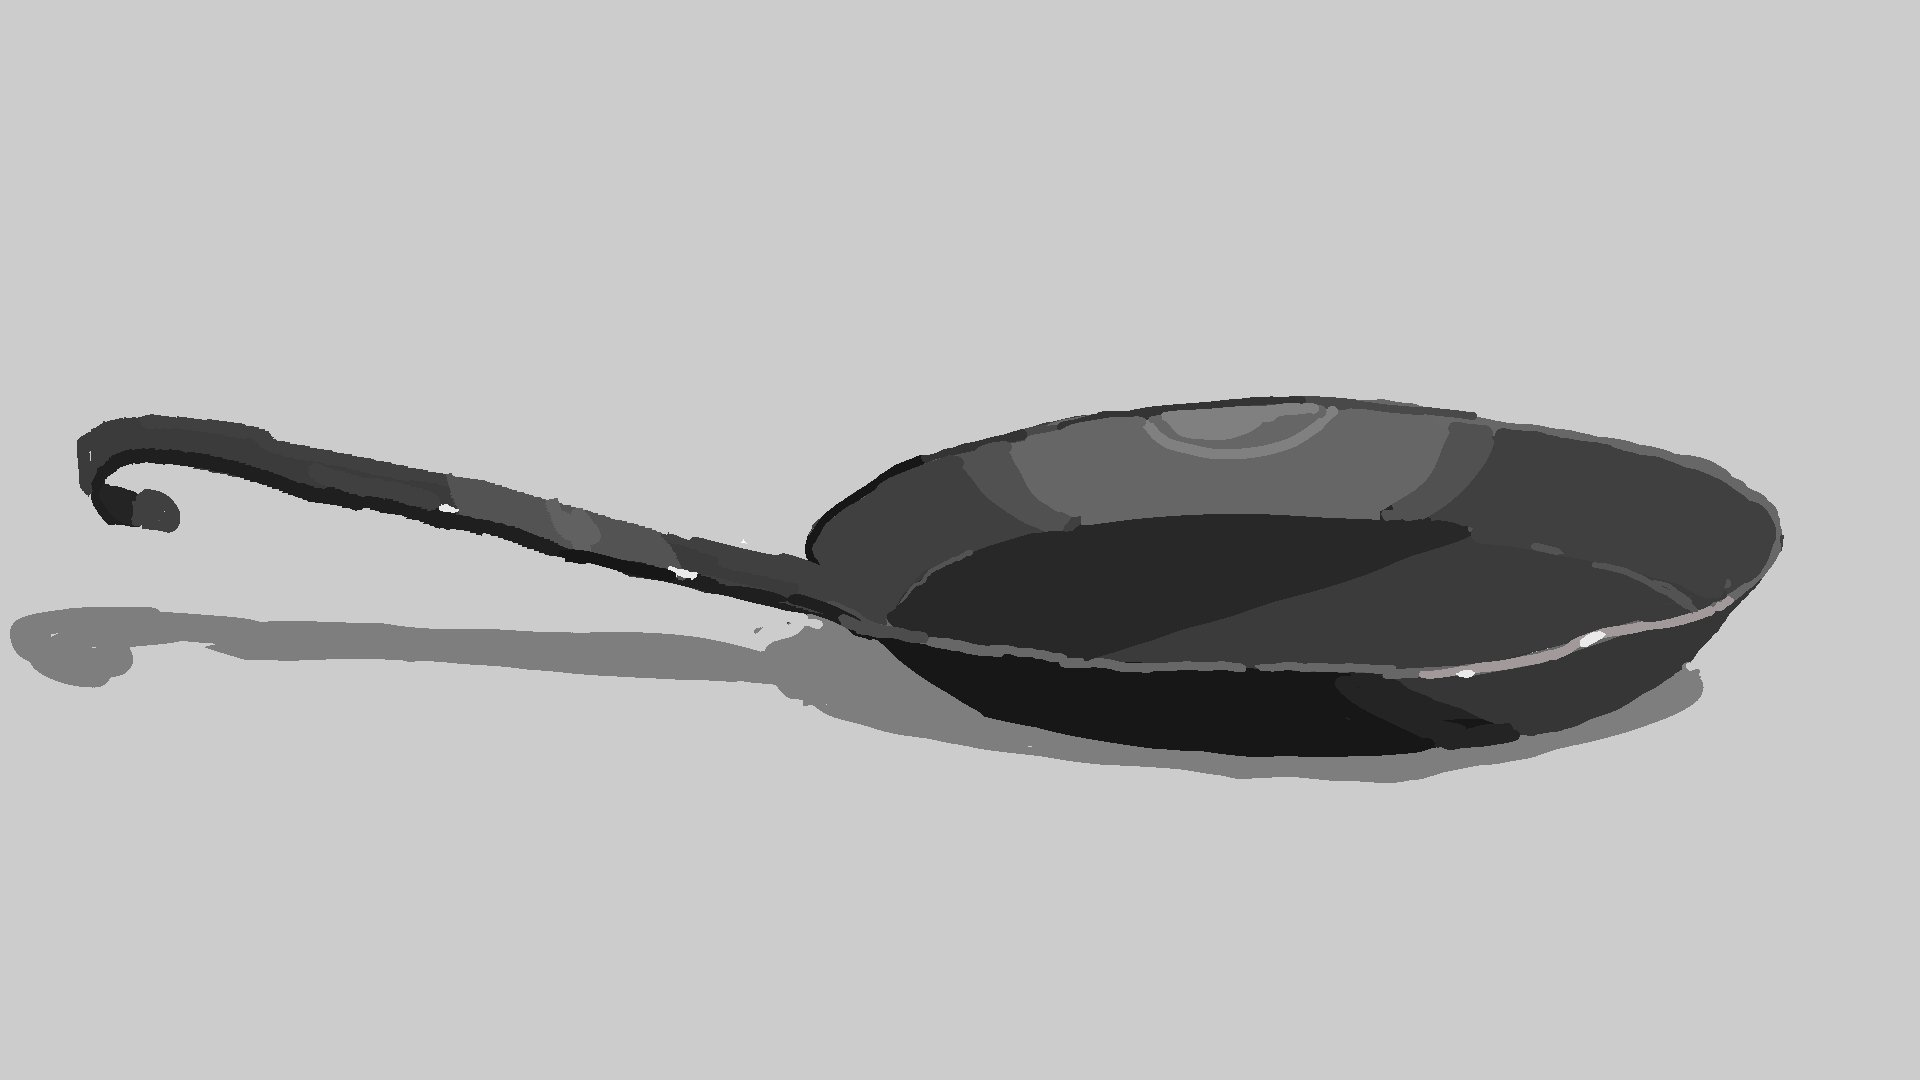
\includegraphics[scale=0.1]{pan.jpg}
\caption{A pan}
\end{figure}


\newpage
\section{Gradients and Directional Derivatives}
With $f:\mathbb{R}^3\rightarrow\mathbb{R}$, the \underline{gradient of f} is the derivative, thought of as a vector.
\[\nabla f(x,y,z)=(\frac{\partial f}{\partial x}(x,y,z),\frac{\partial f}{\partial y}(x,y,z),\frac{\partial f}{\partial z}(z,y,z))\]

\subsection*{Example}
\[f(x,y,z)=xy-z^2\]
\[\nabla f(x,y,z)=(y,z,-2z)\]
\[\nabla f(1,1,0)=(0,1,0)\]

$\nabla f$ gives us a lot of information we can use.\\
Definition: Let $f:\mathbb{R}^3\rightarrow\mathbb{R}$ be a scalar valued differentiable funciton, and let $\vec{v},\vec{w}$ be in $\mathbb{R}^3$

The directional derivative of $f$ at $\vec{v}$ in the direciton of $\vec{w}$ be
\[ i < \frac{\partial f}{\partial t}(\vec{v}+t\vec{w})(0)\]
$\vec{v}+t\vec{w}$ is the line through $\vec{v}$ in the $\vec{w}$ direction.

\subsection*{Theorem}
\[\frac{\partial f}{\partial t}(\vec{v}+t\vec{w})(0) = \overbrace{\nabla f(\vec{v})) \cdot \vec{w}}^{\mbox{the dot product}}\]
\begin{center}
    This is the application of the chain rule. 
\end{center}
\subsection*{Example}
\[f(x,y,z)=x^2 e^{-yz}\]
Compute the directional derivative @ $(1,0,0)$ in the direction of $(1,1,1)$
\[\nabla f(x,y,z)=(2xe^{-yz},-zx^2 e^{-yz},-yx^2 e^{-yz})\]
\[\nabla f(1,0,0)=(2\cdot 1e^0 ,0,0)\]
\[\nabla f(1,0,0)\cdot  (1,1,1)=(2,0,0)\cdot (1,1,1)=2\]
\subsection*{Remark}
What does this mean?

The directional derivative approximates $\nabla f$ if you move from $(1,0,0)+(1,1,1)=(2,1,1)$

\subsection*{Exercise}
\[g(x,y,z)=x^{2}y+z\cos(2\pi x)\]
Compute the directional derivative of $g$ @ $(1,2,3)$ in the direction of $(-1,0,1)$

\[\nabla g(x,y,z) = (2xy+(-2\pi z\sin(2\pi x)),x^2+0,\cos(2\pi x))\]
\[\nabla g(1,2,3)= (4+(-2\pi (3)\sin(2\pi)), 1, \cos(2\pi))\]
\[=(4-6\pi (0),1,0)=(-4+0+0+1)=3\]

\section{Geometric Interpretation of the Gradient}
\[f:\mathbb{R}^3\rightarrow\mathbb{R} \mbox{ is differentiable and scalar valued}\]
\[\nabla f(a,b,c) = \mbox{ a 3D vector}\]

$\nabla f(a,b,c)$ is a normal vector to the tangent plane at a level set. 

\subsection*{Theorem}
If $\nabla f(a,b,c)\neq (0,0,0)$, then the gradient is normal to the tangent plane of the level set of $f$ @ $(a,b,c)$\\
Consequently, the equation for the tangent plane of the level set at $(a,b,c)$ is 
\[\nabla f(a,b,c)\cdot ((x,y,z)-(a,b,c))=0\]

\subsection*{Example}
Consider the ellipsoid $9x^2+2y^2+2z^2=25$.
What is the equation for the tangent plane at $(1,2,2)$?

$f(x,y,z) = 9x^2+2y^2+2z^2=25$ at level 25.
\[\nabla f(x,y,z)=(18x,4y,4z)\]
\[\nabla f(1,2,2)=(18,8,8)\]

\[(18,8,8)\cdot ((x,y,z)-(1,2,2)=0)\]
\[18(x-1)+8(y-2)+8(z-2)=0\]

\subsection*{Theorem}
If $f$ is differentiable and $\nabla f(a,b,c) \neq 0$, then $\nabla f(a,b,c)$ is a normal vector to the tangent plane to the level set.

\subsection*{The Equation for Plane P}

\[\nabla f(a,b,c)\cdot ((x,y,z)-(a,b,c))=0\]
We can "visualize" the gradient as a vector at each point, creating a "vector field" on the graph.

\begin{figure}[h!]
    \centering
    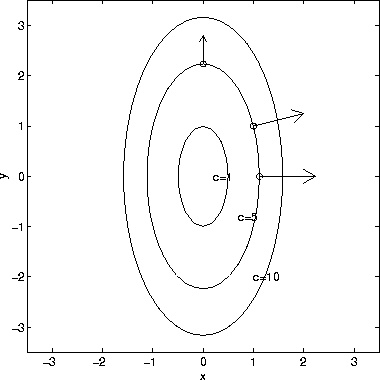
\includegraphics[scale = 1]{vectorField.jpg}
    \caption{A vector field}
    \label{}
\end{figure}
\subsection*{Theorem}
The gradient points in the direction where the function is increasing the greatest.\\
$-\nabla f(a,b) $ is the direction where the function is decreasing the greatest.
\section{Iterated Partial Derivatives}
\subsection*{Definition}
Let $f:\mathbb{R}^3\rightarrow\mathbb{R}$\\
We say f is twice continuously differentiable, or $c^2$

\[\frac{\partial f}{\partial x},\frac{\partial f}{\partial y},\frac{\partial f}{\partial z} \mbox{ are all differentiable}\]
\begin{center}
    and
\end{center}
\[\frac{\partial^2 f}{\partial x^2}=\frac{\partial \frac{\partial f}{\partial x}}{\partial x},\frac{\partial^2 f}{\partial y^2},\frac{\partial^2 f}{\partial z^2},\frac{\partial^2 f}{\partial x \partial y},\frac{\partial^2 f}{\partial y \partial x},\frac{\partial^2 f}{\partial y \partial z},\frac{\partial^2 f}{\partial z \partial y},\frac{\partial^2 f}{\partial x \partial z}, \frac{\partial^2 f}{\partial z \partial x}\]
\begin{center}
    are all differentiable.
\end{center}

\subsection*{Theorem}
If $f:\mathbb{R}^3\rightarrow\mathbb{R}$ is $c^2$, then 
\[\frac{\partial^2 f}{\partial x \partial y} = \frac{\partial^2 f}{\partial y \partial x}\mbox{ (Also true for } \frac{\partial^2 f}{\partial x\partial z}\mbox{ and }\frac{\partial^2 f}{\partial y \partial z}\]

\subsection*{Example}
\[f(x,y) = \cos (xy^2)\]
\[\frac{\partial f}{\partial x} = -y^2\sin(xy^2)\qquad \frac{\partial f}{\partial y}=-2xy\sin(xy^2)\]
\[\frac{\partial^2 f}{\partial x^2}=-y^4\cos(xy^2)\qquad \frac{\partial^2 f}{\partial y^2}=-4x^2y^2\cos(xy^2)\]
\[\frac{\partial^2 f}{\partial y \partial x} = -2y\sin(xy^2) - 2xy^3\cos(xy^2) = \frac{\partial^2 f}{\partial x \partial y}= -2y\sin(xy^2)-2xy^3\cos(xy^2)\]

\subsection*{Exercise}
Compute all the 2nd derivatives

1) $f(x,y) = \log(x+2y)$
\[\frac{\partial f}{\partial x} = \frac{1}{x+2y}\qquad \frac{\partial f}{\partial y}=\frac{2}{x+2y}\]

\[\frac{\partial^2 f}{\partial x^2}=\frac{x+2y(0)-(x+2y)}{(x+2y)^2}=\frac{-1}{x+2y}\]
\[\frac{\partial^2 f}{\partial y^2}=\frac{-2}{(x+2y)^2}\]
\[\frac{\partial^2 f}{\partial y \partial x}= \frac{\partial}{\partial y}(x+2y)^{-1}=\frac{-2}{(x+2y)^2}\]
\[\frac{\partial^2 f}{\partial x \partial y}= \frac{\partial}{\partial x}\frac{2}{x+2y}=\frac{-2}{(x+2y)^2}\]
\newpage

2) $g(x,y)=x^{3}y+2y^2$
\[\frac{\partial f}{\partial x}=3x^{2}y\qquad \frac{\partial f}{\partial y}=x^3+4y\]
\[\frac{\partial^2 f}{\partial x^2}=6xy\qquad \frac{\partial^2 f}{\partial y^2}=4\]
\[\frac{\partial^2 f}{\partial y \partial x}=\frac{\partial}{\partial y}(3x^2y)=3x^2\qquad \frac{\partial^2 f}{\partial x \partial y}=3x^2\]

\section{Subscript Notation}
\[\frac{\partial f}{\partial x}=f_x\qquad \frac{\partial^2 f}{\partial x^2}=f_{xx} =f_{x^2}\]
\[\frac{\partial^2 f}{\partial x \partial y}= f_{xy}\qquad \frac{\partial^2 f}{\partial y^2}=f_y^2\]

\end{document}